\documentclass{article}
\usepackage[utf8]{inputenc}
\usepackage{amsmath, amssymb}
\usepackage{tikz}
\usetikzlibrary{patterns}

\usepackage{geometry}
\geometry{letterpaper, margin=2cm}
\begin{document}
	
	\section*{Problema 3: Intervenciones terapéuticas}
	
	\subsection*{a) Diagrama de Venn}
	
	Sea $U = \{P1, P2, \dots, P20\}$ el conjunto de todas las personas registradas.  
	Los conjuntos son:
	
	
	\[
	R = \text{Regulación emocional}, \quad
	C = \text{Entrenamiento cognitivo}, \quad
	H = \text{Habilidades sociales}
	\]
	
	\begin{center}
		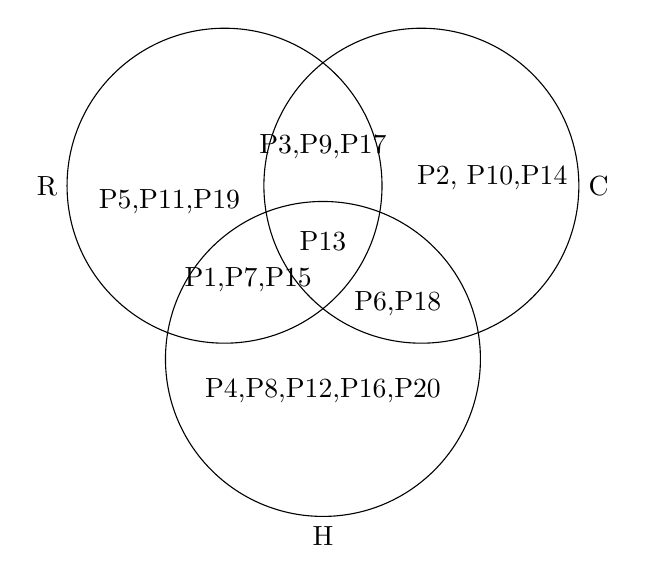
\begin{tikzpicture}
			% Círculos
			\draw (0,0) circle (2cm) node[left=2cm] {R};
			\draw (2.5,0) circle (2cm) node[right=2cm] {C};
			\draw (1.25,-2.2) circle (2cm) node[below=2cm] {H};
			
			% Solo R
			\node at (-0.7,-0.2) {P5,P11,P19};
			% Solo C
			\node at (3.4,0.1) {P2, P10,P14};
			% Solo H
			\node at (1.25,-2.6) {P4,P8,P12,P16,P20};
			% R ∩ C
			\node at (1.25,0.5) {P3,P9,P17};
			% R ∩ H
			\node at (0.3,-1.2) {P1,P7,P15};
			% C ∩ H
			\node at (2.2,-1.5) {P6,P18};
			% R ∩ C ∩ H
			\node at (1.25,-0.7) {P13};
		\end{tikzpicture}
	\end{center}
	
	\subsection*{b) Conjunto A}
	
	
	
	\[
	A = \{x \in U \mid x \text{ participa exactamente en dos intervenciones}\}
	\]
	
	
	
	Por extensión:
	
	
	\[
	A = \{P1, P3, P6, P7, P9, P15, P17, P18\}
	\]
	
	
	
	Cardinalidad:
	
	
	\[
	|A| = 8
	\]
	
	
	
	\subsection*{c) conjunto de personas que participan sólo en Habilidades Sociales, o participan simultáneamente en Regulación Emocional y Entrenamiento Cognitivo:} 
		
	\quad 
	
	Primero Calculamos: el conjunto de personas que participan sólo en Habilidades Sociales:
	
	
	\[
	H-(R\cup C)=\{P4, P8, P12, P16, P20\}
	\]
	
	
	
	Ahora calculamos el conjunto de personas que participan simultáneamente en Regulación Emocional y Entrenamiento Cognitivo:
	
	\[
	R\cap C= \{P3, P9, P13, P17\}
	\]
	
	
	
	Por lo tanto el conjunto solocitado escrito por extensión es:
	
	
	\[
	 [H-(R\cup C)]\cup [(R\cap C)]= \{P3, P4, P8, P9, P12, P13, P16, P17, P20\}
	\]
	
\end{document}
